\documentclass[a4paper]{article}
\usepackage[a4paper]{geometry}

\newcommand{\irace}{\texttt{irace}\xspace}
\newcommand{\iraceversion}{0.9\xspace}

\providecommand{\IridiaTrCover}[1][]{}
%\usepackage{IridiaTrCover}
\newcommand{\techrep}{2011-004}
\newcommand{\techdate}{February 2011}
\newcommand{\revdate}{February 2011}
\newcommand{\ifIridiaTrElse}[2]{#1}
\newcommand{\IridiaTrOnly}[1]{#1}
\usepackage{hyperref}

\usepackage{algorithm,algorithmic}
\usepackage{amsmath,amsfonts,amssymb}
\usepackage[numbers,sort]{natbib}
\usepackage{xspace}
\usepackage{enumitem}
\usepackage{booktabs}
\usepackage{tabularx}
\usepackage{url}
\usepackage{ifthen}
\usepackage{graphicx}


\providecommand{\email}[2]{\normalsize\href{mailto:#1@#2}{\textsf{#1}\textrm{@}\textsf{#2}}}
\newcommand{\true}{\textsc{true}}
\newcommand{\false}{\textsc{false}}
\newcommand{\NULL}{\textsc{null}}
\newcommand{\assign}{\ensuremath{:=}}
\newcommand{\procedure}[1]{\textsf{#1}}
\newcommand{\ie}{i.e.}% id est  --       that is
\newcommand{\eg}{e.g.}% exempli gratia -- for example
\newcommand{\etal}{et al.}% et alii -- and others
\newcommand{\mcol}{\multicolumn}
\newcommand{\cmnt}[1]{\footnote{\noindent\textbf{[ #1 ]}}}
\newcommand{\MANUEL}[1]{{\footnotesize\noindent\textbf{[~MANUEL: #1~]}}}
\newcommand{\THOMAS}[1]{\footnote{\noindent\textbf{[ THOMAS: #1 ]}}}
\newcommand{\hide}[1]{}
\newcommand{\aR}{\textsf{R}\xspace}
\newcommand{\IFRACE}{\text{I/F-Race}\xspace}
\newcommand{\FRACE}{\text{F-Race}\xspace}
\newcommand{\iter}{\ensuremath{i}\xspace}
\newcommand{\Budget}{\ensuremath{B}\xspace}
\newcommand{\Budgeti}{\ensuremath{\Budget_{\iter}}\xspace}
\newcommand{\Bused}{\ensuremath{\Budget_\text{used}}\xspace}
\newcommand{\Ncand}[1][]{\ensuremath{N_{#1}}\xspace}
\newcommand{\Mui}{\ensuremath{\mu_{\iter}}\xspace}
\newcommand{\Nparam}{\ensuremath{{N^\text{param}}}\xspace}
\newcommand{\Niter}{\ensuremath{N^\text{iter}}\xspace}
\newcommand{\tEstimate}{\ensuremath{\hat{t}}\xspace}
\newcommand{\Nmin}{\ensuremath{N^\text{min}}\xspace}
\newcommand{\Nsurv}{\ensuremath{N^\text{surv}}\xspace}
\newcommand{\Nelite}{\ensuremath{N^\text{elite}}\xspace}
\newcommand{\Nnew}{\ensuremath{N^\text{new}}\xspace}
\newcommand{\Celite}{\ensuremath{\Theta^\text{elite}}\xspace}
\newcommand{\cparent}{\ensuremath{\theta^\text{parent}}\xspace}

\newcommand{\defparameter}[4][]{%
%% How to use the command:
% Parameter with one short switch: \defparameter[short]{paramName}{long}{default}
% Parameter without short switch:  \defparameter{paramName}{long}{default}
\hypertarget{opt:#2}{}\ifthenelse{\equal{#1}{}}{~\\ \noindent\textbf{#2\quad  \quad \texttt{--#3}\quad \texttt{#4} \\ \noindent}}%
  {~\\ \noindent\textbf{#2\quad \texttt{-#1} \quad \texttt{--#3}\quad \texttt{#4} \\ \noindent}}%
}
\newcommand{\parameter}[1]{\hyperlink{opt:#1}{\texttt{#1}}}

\begin{document}

\title{The \irace Package:\\ Iterated Race for Automatic Algorithm Configuration}

\author{
  \begin{minipage}[c]{0.9\linewidth}
    \begin{center}
      \begin{tabular*}{0.7\linewidth}{@{\extracolsep{\fill}}lr}
        Manuel L\'opez-Ib\'a\~nez &\email{manuel.lopez-ibanez}{ulb.ac.be} \\    
        J\'er\'emie Dubois-Lacoste & \email{jeremie.dubois-lacoste}{ulb.ac.be} \\               
        Thomas St\"utzle & \email{stuetzle}{ulb.ac.be} \\              
        Mauro Birattari & \email{mbiro}{ulb.ac.be} \\                 
      \end{tabular*}\\[1.5ex]
      \normalsize\emph{IRIDIA, CoDE, Universit\'e Libre de Bruxelles, Brussels, Belgium}\\
      Contact: \email{irace}{iridia.ulb.ac.be}
    \end{center}
  \end{minipage}}

\date{\revdate}

\IridiaTrCover[%
  author={%
Manuel \textsc{L\'opez-Ib\'a\~nez} \and J\'er\'emie \textsc{Dubois-Lacoste}%
\and Thomas \textsc{St\"utzle} \and Mauro \textsc{Birattari}
},
  date=\techdate,
  number=\techrep]%,
%  revdate=\revdate,
%  history=\revhistory]

\maketitle

\begin{abstract}
  The program \irace implements the \emph{iterated racing} procedure,
  which is an extension of the Iterated F-race procedure (\IFRACE).
  Its main purpose is to automatically configure optimization
  algorithms by finding the most appropriate settings given a set of
  instances of an optimization problem. It builds upon the
  \texttt{race} package by Birattari and it is implemented in
  \aR. This revision documents \irace version \iraceversion. The
  latest version of the \irace software is available at \url{http://iridia.ulb.ac.be/irace}.
\end{abstract}

\section{Introduction}

The program \irace implements the \emph{iterated racing} procedure,
which is an extension of the Iterated F-race procedure (\IFRACE)
proposed by \citet{BalBirStu07} and later developed by
\citet{BirYuaBal2010:emaoa}. \irace is implemented in
\aR~\citep{Rmanual} and it builds upon the \texttt{race} package by
\citet{Birattari09tuning,IRIDIA-2003-037}.
%
The main purpose of \irace is to \emph{automatically configure
  optimization algorithms} by finding the most appropriate settings
given a set of instances of an optimization problem. Many optimization
algorithms have a number of configurable parameters, and their
performance on a particular problem often depends on the particular
settings of these parameters. This is particularly true in
metaheuristics, that is, general-purpose solvers such as ant colony
optimization, evolutionary algorithms and other stochastic local
search methods~\citep{HooStu05sls-mk,Birattari09tuning}. Moreover,
complex algorithms may be automatically designed by finding a
particular configuration of a framework composed by alternative design
choices and complementary algorithmic
components~\citep{KhuXuHooLey2009:satenstein,IRIDIA-2011-003}.

The scenario that \irace addresses is usually described as
\emph{offline configuration}~\citep{Birattari09tuning}, that is, there
are two clearly delimited phases. In a primary tuning phase, an
algorithm configuration is chosen given a set of tuning instances
representative of a particular problem. In a secondary production (or
testing) phase, the chosen algorithm configuration is used to solve
unseen instances of the same problem. The goal is to find, during the
tuning phase, an algorithm configuration that minimizes some cost
measure over the set of instances that will be seen during the
production phase.

Offline tuning is frequently performed ad-hoc by algorithm designers
as a result of trial-and-error runs. More formal methods involve the
use of experimental design techniques~\citep{AdeLag06tuning},
evolutionary algorithms~\citep{NanEib2006gecco} and local
search~\citep{HutHooLeyStu2009jair}. \citet{Birattari09tuning} proposed
an automatic configuration approach, \FRACE, based on \emph{racing}
and Friedman's non-parametric two-way analysis of variance by
ranks. This proposal was later improved by performing several
iterations of \FRACE that successively refine a probabilistic model of
the parameter space. The resulting automatic configuration approach
was called Iterated F-race
(\IFRACE)~\citep{BalBirStu07,BirYuaBal2010:emaoa}. Although a formal
description of the \IFRACE procedure is given in the original
publications, no implementation of it has been publicly available.
The \irace package implements a general \emph{iterated racing}
procedure, which includes, as a special case, \IFRACE.


The \irace software presented here has already been extensively tested
in several research projects. \citet{IRIDIA-2010-022,DubLopStu2011cor}
used \irace for tuning the parameters of several iterated greedy (IG)
variants for various objectives in the permutation flow-shop problem
(PFSP). \citet{LopStu2010:ants} automatically configured a flexible
ant colony optimization framework for the bi-objective travelling salesman
problem (bTSP). \citet{MonAydStu2011soco} designed an incremental particle swarm optimization algorithm for large-scale continuous problems by means of automatic configuration.
% Lopez-Ibanez \& Blum configured beam-aco for the TSPTW.  Paola,
% MarcoMontes, TP+PLS, Saifulla, Franco,\footnote{MANUEL: I will
%   update these references last.}
%
These examples demonstrate the potential of automatic configuration of
algorithms, and the profound impact it will have on the way
optimisation algorithms are designed and evaluated in the future.


\section{Automatic Configuration and \IFRACE}\label{sec:prelim}

\subsection{The algorithm configuration problem}\label{sec:algoconf}

\citet{Birattari09tuning} provides a more general and comprehensive
definition of the automatic configuration problem. For brevity, we
will restrict here to a simpler definition that is sufficient for our
purposes.

A parametrized algorithm is an algorithm with $\Nparam$ parameters, $X_d$,
$d=1,\dotsc,\Nparam$, and each of them may take different values (settings).
%$X_d = \{x_d\}$. 
A configuration of the algorithm $\theta$ is a unique assignment of
values to parameters $\theta=\{x_1,\dotsc,x_\Nparam\}$, and $\Theta$
denotes the possibly infinite set of all configurations of the
algorithm.

When considering a problem to be solved by this parametrized
algorithm, the set of possible instances of the problem may be seen as
a set $\mathcal{I}$ from which instances to be solved are
sampled. We are also given a cost measure $\mathcal{C}\colon \Theta
\times \mathcal{I} \to \mathbb{R}$, where $\mathcal{C}(\theta, i)$
measures the quality of configuration $\theta \in \Theta$ on instance
$i \in \mathcal{I}$. Since the algorithm may be stochastic, this cost
measure is often a random variable and the value $c(\theta, i)$ is a
realization of the random variable $\mathcal{C}(\theta, i)$. The cost
value may be the best objective function value found within a given
computation time, or, perhaps, the deviation from the optimum value if
the latter is known. In the case of decision problems, it may
correspond to the computation required to reach a decision, possibly
bounded by a maximum cut-off time. In any case, the cost measure
assigns a quality value to one run of a particular configuration on a
particular instance. The criterion that we want to optimize when
configuring an algorithm for a problem is a function of the cost of a
configuration over the whole set of instances. In that sense, it is a
statistical parameter $c_\theta$ defined on the subordinate
distribution $\mathcal{C}(\theta) = \mathcal{C}(\mathcal{I} \mid
\theta)$. We can now formally define the automatic configuration
problem as finding the best configuration $\theta^*$ such that:
%
\begin{equation}\label{eq:autoconf}
 \theta^* = \arg\min_{\theta \in \Theta} c_\theta\enspace. 
\end{equation}

The precise value of $c_\theta$ is generally unknown, and it can only
be estimated by sampling from $\mathcal{C}(\theta)$. The particular
definition of $c_\theta$ determines how to rank the configurations
over a set of instances. The most typical definition of $c_\theta$ is
$E[\mathcal{C}(\theta)]$, the expected cost value or mean cost. If the
cost values over different instances are incommensurable, the median
or the sum of ranks may be more meaningful.



\subsection{Classes of parameters}

There are two main classes of  parameters:
\emph{categorical} and \emph{numerical} parameters. Categorical
parameters represent discrete values without any implicit order or
sensible distance measure, whereas numerical parameters have an
implicit order of their values. There are also seemingly categorical
parameters but with an implicit order or distance measure of their
values. An example would be a parameter with three values
$\{$\texttt{low}, \texttt{medium}, \texttt{high}$\}$. Such parameters
are called \emph{ordinal} and are typically handled as numerical
parameters~\citep{BirYuaBal2010:emaoa}. Finally, parameters may be
\emph{subordinate} on other parameters, that is, they are only enabled
when the values of other parameters satisfy a particular
condition. For instance, the tabu list length only matters if tabu search is chosen as the local search algorithm. Subordinate parameters are not the same as
constraints on the values of parameters.  For example, given
parameters $a$ and $b$, a constraint may be that $a < b$. Such
constraints limit the range of values that a certain parameter can
take in dependence of other parameters, whereas subordinate parameters
are either disabled or they have a value according to a predefined
range. In some cases, parameter constraints may be modeled by
replacing one of the parameters by a surrogate parameter, \eg{}, $a'
\in (0,1)$, such that $ a = a' \cdot b$.


\subsection{Racing}

Racing was first proposed in machine learning to deal with the problem
of model selection~\citep{MarMoo1997air}. 
\citet{Birattari09tuning} adapted the procedure for the configuration
of optimization algorithms. A race starts with a finite set of
candidate configurations. At each step of the race, the candidate
configurations are evaluated on a single instance. After each step,
those candidate configurations that perform statistically worse than
the rest are discarded, and the race continues with the remaining
\emph{surviving} configurations. This procedure continues until
reaching a minimum number of surviving configurations, a maximum
number of instances or a pre-defined computational budget. This
computational budget may be an overall computation time or a number of
experiments.

There are several alternatives for selecting which configurations
should be discarded during the race. The \FRACE
algorithm~\citep{Birattari09tuning,BirStuPaqVar02:gecco} relies on the
non-parametric Friedman's two-way analysis of variance by ranks, the
Friedman test, and its associated post-hoc test, as described by
Conover~\citep{Conover99:pns}. Nonetheless, the \texttt{race}
package~\citep{IRIDIA-2003-037} implements various alternatives based
on the paired t-test with and without p-value correction for multiple
comparisons, which are also available in the proposed \texttt{irace}
package.

\subsection{\IFRACE}

The racing approach is particularly effective if the initial set of
configurations is exhaustive. However, it is often the case in
practice that the configuration space is too large to be sampled
effectively. Moreover, the knowledge gathered during the race itself
could be used to sample new candidate configurations. 

\IFRACE was proposed~\citep{BalBirStu07,BirYuaBal2010:emaoa} as an
extension of \FRACE in order to search the configuration space more
effectively by focusing on the most promising configurations. \IFRACE
iterates over a sequence of races, and the candidate configurations
evaluated in each subsequent race depend on the results of previous
races. Candidate configurations are generated by sampling according to
some probability model $P_X$ defined over the parameter space
$X$. Without prior knowledge, the sampling is initially done according
to a uniform distribution. In subsequent iterations, numerical
parameters are sampled according to a normal distribution, whereas
categorical parameters are sampled according to a discrete probability
function. The \irace software that we propose in the next section is
an implementation of iterated racing that includes \IFRACE as a
special case.


\section{Iterated Racing}\label{sec:irace}

In this section, we describe the exact implementation of iterated
race as proposed in the \irace package. Implementation details and setup of the \irace package itself are given in the next section.

An outline of the iterated racing algorithm is given in
Algorithm~\ref{alg:irace}. It requires as input: a set of instances, a
parameter space, a cost function, and a tuning budget ($\Budget$).

\begin{algorithm}[tb]
\caption{Iterated Racing}\label{alg:irace}
\begin{algorithmic}[1]
\REQUIRE $\{I_1,I_2,\dotsc,\} \sim\mathcal{I}$,\newline
parameter space: $X$,\newline
cost measure: $\mathcal{C}\colon \Theta
\times \mathcal{I} \to \mathbb{R}$,\newline
tuning budget: $\Budget$
\STATE $\Theta_1 \sim \procedure{SampleUniform}(X)$
\STATE $\Celite \assign \procedure{Race}$($\Theta_1$, $\Budget_1$)
  \STATE $i \assign 2$
\WHILE{$\Bused \leq \Budget$}
  \STATE $\Theta^\text{new} \sim \textsf{Sample}(X, \Celite)$
\STATE $\Theta_i \assign \Theta^\text{new} \cup \Celite$
\STATE $\Celite \assign \procedure{Race}$($\Theta_i$, $\Budgeti$)
\STATE $i \assign i + 1$
\IF{$i > \Niter$}
\STATE $\Niter \assign i$
\ENDIF
\ENDWHILE
\STATE \textbf{Output:} $\Celite$
\end{algorithmic}
\end{algorithm}

% \begin{algorithm}[tb]
% \caption{\procedure{Race}($\Theta_i$, $\Budgeti$)}\label{alg:race}
% \begin{algorithmic}[1]
% \STATE $s \assign 1$
% \REPEAT
% \FOR{$\theta_k \in \Theta_i$}
% \STATE $\Celite \assign \procedure{Race}$($\Theta_1$, $\Budget_1$)
% \STATE $\Nsurv \assign |\Theta_i|$
% \ENDFOR
% \UNTIL{$\Budgeti < \Nsurv$ \textbf{or} $\Nsurv \leq \Nmin$}
% \STATE \textbf{Output:} $\Celite$
% \end{algorithmic}
% \end{algorithm}

Iterated race requires an estimation of the number of iterations
$\Niter$ (races) that it will execute. The default setting of $\Niter$
depends on the number of parameters with $\Niter = \lfloor 2 +
\log_{2}\Nparam \rfloor$. Each iteration performs one race with a
limited computation budget $\Budgeti = (\Budget - \Bused) / (\Niter -
\iter + 1)$, where $\iter = 1, \dotsc, \Niter$. Each race starts from
a set of candidate configurations $\Theta_\iter$. The number of
candidate configurations is calculated as $|\Theta_\iter|= \Ncand[\iter] =
\lfloor \Budgeti / (\mu + \iter)\rfloor$. Thus, the number of
candidate configurations decreases with the number of iterations,
which means that more evaluations per configuration will be performed
in later iterations. Moreover, increasing the value of $\mu$ also
increases the number of evaluations per candidate configuration. 

\newcommand{\Tfirst}{\ensuremath{T^\text{first}}\xspace}
\newcommand{\Teach}{\ensuremath{T^\text{each}}\xspace}

In the first iteration, the initial set of candidate configurations is
generated by uniformly sampling the parameter space $X$. When a race
starts, each configuration is evaluated on the first instance by means of
the, possibly stochastic, cost measure $\mathcal{C}$. Configurations
are iteratively evaluated on subsequent instances until a number of
instances have been seen ($\Tfirst$). Then, a statistical
test is performed on the results. If there is enough statistical
evidence to identify some candidate configurations as performing worse
than the rest, the worst configurations are removed from the
race, while the rest, the \emph{surviving} candidates, are run on the
next instance. A new statistical test is performed every $\Teach$
instances.
%
The race continues until the budget of the current iteration is not enough to
test all remaining candidate configurations on a new instance
($\Budgeti < \Nsurv$), or when at most $\Nmin$ configurations remain,
$\Nsurv \leq \Nmin$. 
%The value of $\Nmin$ may be specified using
%option \parameter{minNbSurvival}, and the current default is $\Nmin =
%\lfloor 2 + \log_2\Nparam\rfloor$.

At the end of a race, a number $\Nelite_i = \min(\Nsurv, \Nmin)$ of
elite configurations $\Celite$ are selected from the
surviving configurations, by ranking them according to the sum of
ranks or the mean cost, depending on which statistical test is used
during the race. Then, a weight $w_z$ is assigned to each elite
configuration $\theta_z$, $z=1,\dotsc, \Nelite$, according to their
ranks $r_z$:
%
\begin{equation}\label{eq:weight}
  w_z = \frac{\Nelite_i - r_z + 1}{\Nelite_i \cdot (\Nelite + 1) /2}\enspace.
\end{equation}
%
This weight $w_z$ is used for generating new candidate configurations
for the next race. 

In the next race, a number of $\Nnew_i = \Ncand[\iter] - \Nelite_i$ new
candidate configurations are generated. For generating a new
configuration, first one parent configuration is
sampled from the set of elite configurations $\theta_z\sim\Celite$
with a probability proportional to its weight $w_z$. Next, a new value
is sampled for each parameter $X_d$, $d=1,\dotsc,\Nparam$, according
to a distribution that its associated to each parameter of
$\theta_z$. Parameters are considered in the order determined by the
dependency graph of conditions, that is, unsubordinate parameters are
sampled first, those parameters that are subordinate on them are
sampled next if the condition is satisfied, and so on. Moreover, if a subordinate parameter that was disabled in the
parent configuration becomes enabled in the new configuration, then
the parameter is sampled uniformly, as in the initialization phase.

If $X_d$ is a numerical parameter defined within the range of $X_d \in
[\underline{x}_d, \overline{x}_d]$, then a new value is sampled from
the truncated normal distribution $\mathcal{N}(x_d^z, (\overline{x}_d - \underline{x}_d)\cdot\sigma_d^i)$,
such that the new value is within the range.\footnote{%
  For sampling from a truncated normal distribution, we use the
  \texttt{msm} package~\citep{Jac2011jss}.} The mean of the
distribution $x_d^z$ is simply the value of parameter $d$ in the elite
configuration $\theta_z$. The parameter $\sigma_d^i$ controlling the standard deviation of the distribution is initially set to $1$, and it is updated at each iteration before sampling as follows:
%
\begin{equation}\label{eq:sigma}
  \sigma_d^i \assign  \sigma_d^{i-1} \cdot {(\Nnew_i)}^{\frac{1-i}{\Nparam}}
\end{equation}
%
If the numerical parameter is of integer type, we round the sampled
value to the nearest integer. Parameters of ordinal type are
encoded as integers.

If $X_d$ is a categorical parameter with levels $X_d \in \{x_1, x_2,
\dotsc, x_{n_d} \}$, then a new value is sampled from a discrete
probability distribution $\mathcal{P}^{\iter,z}(X_d)$. In the first iteration ($\iter = 1$), $\mathcal{P}^{1,z}(X_d)$ is uniformly distributed over
the domain of $X_d$. In subsequent iterations, it is updated before
sampling as follows:
%
\begin{equation}\label{eq:prob_update}
  \mathcal{P}^{\iter,z} (X_d = x_j) \assign \mathcal{P}^{\iter-1,z} (X_d = x_j)
  \cdot \left(1 - \frac{\iter-1}{\Niter}\right) + \Delta \mathcal{P}
\end{equation}
where 
\begin{equation}\label{eq:2}
  \Delta \mathcal{P} = 
  \begin{cases}
    \dfrac{\iter - 1}{\Niter} & \text{if $x_j = x_z$}\\
    0  & \text{otherwise}\\
  \end{cases}
\end{equation}
%

Finally, the new configurations generated after sampling inherit the
probability distributions from their parents, and a new race is
launched with the union of the new configurations and the elite
configurations.

The algorithm stops if the budget is exhausted ($\Bused > \Budget$) or
if the number of candidate configurations to be generated at the start
of an iteration is not greater than the number of elites ($\Ncand[\iter]
\leq \Nelite_i$), since in that case no new configurations would be
generated. If the iteration counter $\iter$ reaches the estimated
number of iterations $\Niter$, we simply adjust the number of
iterations accordingly and continue.



\section{Extensions}

We have implemented some extensions that were not proposed in the
original publications.

\subsection{Initial configurations}

We can seed the iterated race procedure with a set of initial
configurations. In that case, only enough configurations are sampled
to reach $\Ncand[1]$ in total. For how to specify the initial set of configurations, see option \parameter{candidatesFile}.

\subsection{Tuning for computation time}\label{sec:time}

Sometimes the goal is to minimize the computation time required to
perform a task. For example, in decision problems, the goal is to
minimize the time that an algorithm takes to reach an answer. In the
case of complete algorithms that optimally solve an optimization
problem, the goal is to minimize the time to reach the optimal
solution. 

When automatically configuring an algorithm for minimizing computation
time, it is often preferred to define the tuning budget $\Budget$ as a
computation time limit, instead of a maximum number of experiments. In
such case, the budget of each iteration is computed as $\Budgeti =
(\Budget - \Bused) / (\tEstimate_{\iter}\cdot(\Niter - \iter + 1))$,
where $\iter = 1, \dotsc, \Niter$, and $\tEstimate_{\iter}$ is an
estimate of the computation time required by a single run of the
algorithm. The initial value of this estimate is provided by the user,
for example, as a cut-off time after which an algorithm run is stopped
even if no decision has been reached.  In subsequent iterations,
$\tEstimate$ is updated by computing the average time used by the
experiments performed so far.


\subsection{Soft-restart}

Our implementation incorporates a ``soft-restart'' mechanism to avoid
premature convergence. In the original \IFRACE
proposal~\citep{BalBirStu07}, the standard deviation, in the case of
numerical parameters, or the discrete probability of unselected
parameter settings, in the case of categorical ones, decreases at every
iteration. Diversity is introduced by the variability of the
configurations. However, if the tuning converges to a few, very
similar elite configurations in few iterations, the diversity is lost
and new candidate configurations are very similar. Such a premature
convergence wastes the remaining  budget on repeatedly
evaluating very similar configurations, without exploring new
alternatives.

We implemented a ``soft-restart'' mechanism that checks for premature
convergence after generating each new set of candidate configurations. If
premature convergence has occurred, the probabilistic model is
partially reinitialized. We consider that there is premature
convergence when the ``distance'' between two candidate
configurations is zero. The
distance between two configurations is defined as the maximum distance
between their parameter settings, which is defined as follows:

\begin{itemize}
\item If the parameter is subordinate and disabled in both configurations, the distance is zero;
\item if it is disabled in one configuration but enabled in the other,
  the distance is one;
\item if the parameter is enabled in both configurations (or it is not subordinate), then: 

  \begin{itemize}
  \item in the case of numerical parameters (integral or real), the
  distance is the absolute normalized difference between
  their values (the values are rounded up to the number of significant digits specified by the option \parameter{signifDigits}) ;
\item in the case of ordinal and categorical parameters, the distance
  is one if the values are different and zero otherwise.
\end{itemize}
\end{itemize}

When premature convergence is detected, a ``soft-restart'' is applied
by partially reinitializing the probabilistic model. This
reinitialization is applied only to the elite configurations that were
used to generate the candidate configurations with zero distance,
because the other elite configurations may not suffer from premature
convergence, and it would be detrimental to restart their
probabilistic models. In the case of categorical parameters, the
discrete probability model of elite configuration $z$,
$\mathcal{P}^{\iter,z}(X_d)$, is adjusted by modifying each individual
probability value $p \in \mathcal{P}^{\iter,z}(X_d)$ with respect to
the maximum value $p_\text{max} = \max\{\mathcal{P}^{\iter,z}(X_d)\}$
as follows:
%
\[p \assign \frac{0.9 \cdot p + 0.1 \cdot p_\text{max}}{\sum_{p' \in \mathcal{P}^{\iter,z}(X_d)} 0.9 \cdot p' + 0.1 \cdot p_\text{max}}\enspace.\]
%
For numerical and ordinal parameters, the standard deviation of elite configuration $z$, $\sigma_d^{\iter,z}$, is ``brought back'' two iterations, with a maximum limit of its value in the second iteration, as follows:
\[
  \sigma_d^{\iter,z} \assign \min\{ \sigma_d^{\iter,z} \cdot {(\Nnew_i)}^{\frac{2}{\Nparam}},
{(\Nnew_i)}^{\frac{-1}{\Nparam}}\}
\]

After adjusting the probability model of all affected elite
configurations, the set of candidate configurations that triggered the
soft-restart is discarded and a new set of $\Nnew$ configurations is
sampled from the elite configurations. This procedure is applied at
most once per iteration.


\section{The \irace software}\label{sec:setup}

This section describes the requirements, implementation details, and
the setup of the \irace package.


The scheme in Fig.~\ref{fig:irace-scheme} describes how the different
parts of \irace interact with each other. The program \irace requires
three main inputs:

\begin{enumerate}
\item A description of the parameter space $X$, which is provided by a
  file \parameter{parameterFile} that describes the parameters to
  configure, their types, ranges and constraints. The format of this
  file is explained in detail in Section~\ref{sec:paramFile}.

\item The set of tuning instances $\{I_1, I_2, \dotsc\}$, which in
  practice is a finite, hopefully representative, sample of
  $\mathcal{I}$. The particular options for specifying the set of
  tuning instances are given in Section~\ref{sec:instances}.

\item The configuration of \irace itself, which is defined by a number
  of options. These options may be defined in a configuration file or
  in the command line. Table~\ref{tab:options} maps the description of
  iterated racing in the previous section to the configuration options
  in \irace. The complete list of options is given in
  \autoref{appendixA}.
\end{enumerate}

An initial set of configurations may be provided by means of an
optional candidates file (see option \parameter{candidatesFile}). The
evaluation of candidate configurations is performed in two phases by
means of two auxiliary programs called ``hooks''. These hooks are
described in Section~\ref{sec:hooks}. A step-by-step guide of setting
up a new tuning scenario is provided in
Section~\ref{sec:tuning_setup}; examples of tuning scenarios are
given in Section~\ref{sec:applications}.


\begin{figure}[tbp]
  \centering
  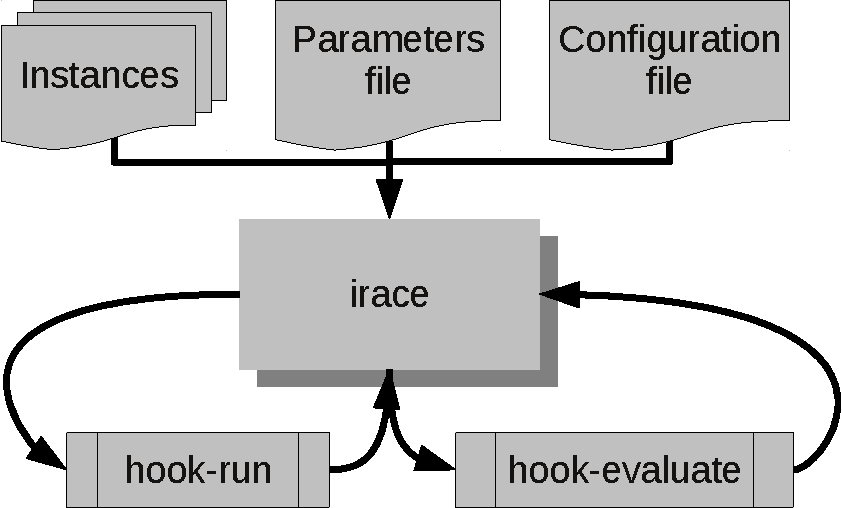
\includegraphics[width=0.6\textwidth]{irace-scheme-crop}
  \caption{Scheme of \irace flow of information.}
\label{fig:irace-scheme}
\end{figure}

\begin{table}[t]
  \centering
  \caption{Configuration options of \irace corresponding to the description of Iterated racing given in Section~\ref{sec:irace}. The full list of options is available in \autoref{appendixA}.}
  \label{tab:options}
  \begin{tabular}[c]{rl}
\toprule
\textbf{Iterated racing parameter}&\textbf{\irace configuration option}\\
\midrule
\Budget     & either \parameter{maxExperiments} or \parameter{timeBudget}\\
$\mathcal{C}$ (cost measure) & \parameter{hookRun} and \parameter{hookEvaluate}, see also Section~\ref{sec:hooks}\\
$\Niter$    & \parameter{nbIterations}\\
$\mu$       & \parameter{mu}\\
$\Nmin$     & \parameter{minNbSurvival}\\
\Tfirst     &\parameter{firstTest} \\
\Teach      & \parameter{eachTest} \\
Statistical test & \parameter{testType}\\
$\tEstimate_1$ & \parameter{timeEstimate}, see also Section~\ref{sec:time}\\
\bottomrule
  \end{tabular}
\end{table}



\subsection{Requirements}

\begin{itemize}
\item \aR version $\geq 2.10$ (\url{http://www.r-project.org/}).
\item The wrappers \texttt{irace} and \texttt{parallel-irace} require GNU Bash.
\item The option \texttt{--parallel} requires the \texttt{multicore} package~\citep{R:multicore}.
\item The option \texttt{--mpi} requires the \texttt{Rmpi} package~\cite{R:Rmpi}.

\item Cluster-mode (\texttt{--sge-cluster 1}) requires Grid Engine
  commands \texttt{qsub} and \texttt{qstat}. The command \texttt{qsub}
  should return a message that contains the string: \texttt{"Your job
    JOBID"}. The command \texttt{"qstat -j JOBID"} returns nonzero if
  JOBID has finished, otherwise it should return zero.
\end{itemize}


\subsection{Installation}

Installation simply involves copying the files to a particular
location, e.g., \texttt{/usr/irace/}. To invoke \irace, just either
add its path to the environment variable \verb|$PATH|, or invoke it
explicitly as \texttt{/usr/irace/irace}.




\subsection{Tuning Instances}\label{sec:instances}

The set of tuning instances $\{I_1, I_2, \dotsc\}$, which in
practice is a finite, hopefully representative, sample of
$\mathcal{I}$, is read from \parameter{instanceFile}. The path given
by option \parameter{instanceDir} will be prefixed to them, although
these instances do not need to correspond to physical files. If the
option \parameter{instanceFile} is not set, then \irace considers all
files found in \parameter{instanceDir}, and recursively in its
subdirectories, as tuning instances. The order in which instances
are considered by \irace is randomized if the
option \parameter{sampleInstances} is enabled. Otherwise, the order is
the same given in the \parameter{instanceFile}, if this option is set,
or in alphabetical order if there is no \parameter{instanceFile}.

\subsection{Configuration File}\label{sec:configFile}
 
The configurable parameters of \irace can be defined in a
configuration file or on the command-line. The full list of
configurable parameters is given in
\autoref{appendixA}. If the same parameter is defined
both in the configuration file and on the command-line, the value
given on the command-line has preference. If a parameter is not set
neither in the configuration file nor on the command-line, the default
value is used.

The configuration file uses the \aR syntax, for example:
%
\begin{verbatim}
     paramNumeric <- 1
     paramString  <- "a string"
\end{verbatim}
%
Moreover, anything in a line after the symbol `\texttt{\#}' is ignored.

Many of the parameter exposed affect the internals of \irace and we
advise to not change their default values without fully understanding
their effects.


% The behavior of \irace is quite open through the possible setting of
% the numerous parameters listed in \hyperref[appendixA]{Appendix A}. On
% the one hand, it allows the user to easily define a configuration for
% the tuner that corresponds exactly to the specificities of its program
% and tuning scenario. On the other hand, some combinations of values
% could lead to unconsistent behaviors, or even to unexpected
% termination of the tuner. We advise the user to not change a parameter
% value from the default one unless he fully understands the effects of
% such a parameter.


\subsection{Parameters file}\label{sec:paramFile}

The parameters of the algorithm to be tuned are described in a
\emph{parameter file}, see the example in \verb|templates/parameters.tmpl|. Each line defines a configurable parameter:
%
\begin{verbatim}
     <name> <switch> <type> <range> [ | <condition> ]
\end{verbatim}
%
where each field is defined as follows:
%
\begin{center}
\renewcommand{\arraystretch}{1.2}
  \begin{tabularx}{0.98\linewidth}{@{}rX}
    \texttt{<name>} & The name of the parameter as an unquoted
    alphanumeric string,
    for instance \texttt{ants}.\\
    \texttt{<switch>}& The command-line switch used to pass the value of this parameter to \parameter{hookRun}, for instance \texttt{"--ants "}. The value of the parameter is concatenated \emph{without separator} to the switch string when invoking \parameter{hookRun}.\\

    \texttt &The type of the parameter, either
    \textit{integer},
    \textit{real}, \textit{ordinal} or \textit{categorical}, given as a single letter: \texttt{i}, \texttt{r}, \texttt{o} or \texttt{c}. \\
    \texttt &The range or set of values of the parameter.\\
    \texttt& An optional \emph{condition} that
    determines whether the parameter is enabled or disabled. If the
    condition evaluates to false, then no value is assigned to this
    parameter, and the corresponding switch is not passed
    to \parameter{hookRun}. The condition must be a valid \aR logical
    expression. The condition may contain the name of other parameters
    as long as the dependency graph does not contain any
    cycle. Otherwise, \irace will detect the cycle and stop with an error.\\
  \end{tabularx}
\end{center}

\paragraph{Parameter types and range.}
Parameters can be of four types:
%
\begin{itemize}
\item \textit{Real} parameters are numerical parameters that can take
  any floating-point values within a given range. The range is
  specified as an interval \texttt{(<lower bound>,<upper
    bound>)}. This interval is closed, that is, the parameter value
  may eventually be one of the bounds. The possible values are rounded
  to a number of \emph{significant digits} specified by
  option \parameter{signifDigits}. For example, given the default
  value number of significant digits of $4$, the values $0.12345$ and
  $0.12341$ are both rounded to $0.1234$. However, the values
  $0.00001$ and $0.00005$ remain the same.

\item \textit{Integer} parameters are numerical parameters that can
  take only integer values within the given range. The range is
  specified as for real parameters.

\item \textit{Categorical} parameters are defined by a set of possible
  values specified as \texttt{(<value 1>, ..., <value n>)}. The values
  are quoted or unquoted character strings. Empty strings and strings
  containing commas or spaces must be quoted.

\item \emph{Ordinal} parameters are defined by an \emph{ordered} set
  of possible values in the same format as for categorical parameters.

\end{itemize}


\paragraph{Subordinate parameters.} 
A subordinate parameter is one that is enabled or disabled depending
on the values of other parameters. A parameter is marked as
subordinate by adding the character \texttt{'|'} followed by an \aR
expression involving the names of other parameters. This expression
must return \texttt{TRUE} when the parameter should be enabled, and
\texttt{FALSE} otherwise. Examples of operators that are valid in a condition are relational operators 
(\texttt{<, >, <=, >=, ==, !=}) and the logical operators: \texttt{!~\textrm{(not)}, \&\&~\textrm{(logical-and)},
  ||~\textrm{(logical-or)}}. Another useful operator is
\texttt{\%in\%}, which returns \texttt{TRUE} if its left operand matches any
element of its right operand. See the example below.

\paragraph{Example.}

We describe now in detail the example provided in \texttt{templates/parameters.tmpl}
\begin{verbatim}
param1     "--param1 "          i  (1, 10) | mode %in% c("x1", "x2")
param2     "--param2 "          c  (1, 10) | mode == "x1" && real < 3.5
mode       "--"                 c  ("x1" ,"x2", "x3")
p.real     "--paramreal="       r  (1.5, 4.5)
p.ordinal  "--level="           o  ("low", "medium", "high", "very high")
#unused    "-u "                c  (1, 2, 10, 20)
\end{verbatim}

In this example, \texttt{param1} is an integer parameter in the interval $[1,10]$, and it
is only enabled when parameter \texttt{mode} takes values \texttt{x1} or \texttt{x2}.  Parameter \texttt{param2} is a
categorical parameter with only two values, either \texttt{"1"} or \texttt{"10"}. It is
only enabled when parameter \texttt{mode} takes the value \texttt{x1} and parameter \texttt{p.real}
has a value lower than 3.5. Parameter \texttt{mode} is a categorical parameter
with three possible values. Given its corresponding switch, these values are translated into \texttt{"--x1"}, \texttt{"--x2"} and \texttt{"--x3"} when invoking
\parameter{hookRun}. Parameter \texttt{p.real} may take any real value
within the interval $[1.5, 4.5]$ (subject to the number of significant
digits specified by \parameter{signifDigits}). Parameter
\texttt{p.ordinal} is an ordinal variable.  Finally,
parameter \texttt{unused} is commented out, and, hence, ignored.

It is possible to specify a categorical parameter with a single
value. This parameter is added to the command line as usual when
invoking \parameter{hookRun}, subject to any possible condition, but
it is never sampled and it is not counted by $\Nparam$.


\subsection{Hook files}\label{sec:hooks}

The evaluation of the candidate configurations is done in two
phases. In the first phase, the program specified by the
option \parameter{hookRun} is invoked for each candidate
configuration, passing as arguments: the instance name, a numeric
identifier, and the command-line parameters of the candidate
configuration. The numeric identifier uniquely identifies a
configuration within a race (but not across the races in a single
iterated race). The command line is constructed by appending to each
parameter switch, \emph{without separator}, the value of the
parameter, following the order given in the parameter file. If the
options \parameter{parallel}, \parameter{mpi}
or \parameter{sgeCluster} are enabled, the calls
to \parameter{hookRun} happen in parallel. The
program \parameter{hookRun} should not have any output and it should
exit with a value of zero.  Once all calls to \parameter{hookRun} for
the current instance have finished, the results are evaluated using
the program specified by option \parameter{hookEvaluate}.

In this second phase, the program 
\parameter{hookEvaluate} is invoked for each candidate configuration
in order of increasing candidate number. The parameters
of \parameter{hookEvaluate} are the instance name, the numeric
identifier and the total number of candidate configurations alive at
this point of the race. The program \parameter{hookEvaluate} must
print (only) a real number, which corresponds to the cost measure of
the candidate configuration in the given instance.

The working directory of these programs is set to the execution
directory specified by the option \parameter{execDir}. This allows the
user to execute several runs of \irace in parallel with the same
configuration files without the runs interfering with each other.


\subsection{Tuning Setup}\label{sec:tuning_setup}

The following steps detail how to setup a new tuning environment from scratch:

\begin{enumerate}
\item Create a new directory for storing the configuration of the
  tuning, \eg{}, \texttt{/path/to/tuning/}.

\item Copy the files in the \texttt{templates/} directory to your
  \texttt{/path/to/tuning/} directory.  For each template hook
  (\verb|*.tmpl|) in your \texttt{/path/to/tuning/} directory, remove the
  \verb|'.tmpl'| suffix, and modify them following the instructions in each
  file. In particular, \texttt{tune-main.tmpl} should be adjusted depending on
  your usage (local, cluster, etc).  The hooks should be
  executable. In \verb|tune-conf.tmpl|, uncomment and assign only the
  parameters for which you need a value different than the default
  one. See the examples in \texttt{examples/}.


\item Put the instances in \texttt{/path/to/tuning/Instances/}. As
  described in Section~\ref{sec:instances}, you can
  also create a file that specifies which instances from that directory
  should be run and which instance-specific parameters to use. See
  \texttt{tune-conf.tmpl} and \texttt{instances-list.tmpl} for
  examples.

\item Assuming that \irace is installed in \texttt{/installdir/},
  calling the command \texttt{/installdir/irace} from your tuning
  directory performs one run of \irace. See \autoref{appendixA} for
  additional configuration options. Command-line parameters override
  the configuration specified in the configuration file
  (\texttt{tune-conf}). The command \irace will not attempt to create
  the execution directory (\texttt{execDir}), so it must exist before
  calling irace.

\item For executing several repetitions of \irace in parallel, call
  the program \texttt{parallel-irace.sh} from your tuning directory
  with the number of repetitions. The execution directory of each run
  of irace will be set to ``\texttt{/path/to/tuning/TUNE-dd}'', where
  \texttt{dd} is a number padded with zeroes. Be careful,
  \texttt{parallel-irace.sh} will create these directories from scratch,
  deleting them first if they already exist. Check the help of
  \texttt{parallel-irace.sh} by running it without parameters.
\end{enumerate}


There are three ways to execute the calls to \parameter{hookRun} in parallel:

\begin{enumerate}
\item \texttt{--parallel N}\hspace{2ex} will use the \texttt{multicore} package~\citep{R:multicore} to launch locally
  up to \texttt{N} calls of \parameter{hookRun} in parallel.

  \item \texttt{--mpi 1 --parallel N}\hspace{2ex}  will use the \texttt{Rmpi} package~\cite{R:Rmpi} to launch \texttt{N}
  slaves + 1 master, in order to execute \texttt{N} calls of \parameter{hookRun} in
  parallel. The user is responsible to set up MPI correctly. For an
  example of using MPI mode in an SGE cluster, see \texttt{examples/mpi/}.

\item \texttt{--sge-cluster 1}\hspace{2ex}  will launch as many calls
  of \parameter{hookRun} as possible and use '\texttt{qstat}' to wait
  for cluster jobs. The user \textbf{must} call '\texttt{qsub}'
  from \parameter{hookRun} with the appropriate configuration for
  their cluster, otherwise \parameter{hookRun} will not submit jobs to
  the cluster. In this mode, \irace must run in the submission node,
  and hence, '\texttt{qsub}' should not be used to invoke \irace
  (either directly or through \texttt{tune-main}).  See the examples
  in \texttt{examples/cluster-mode/}.
\end{enumerate}


\section{Examples of Tuning Scenarios}\label{sec:applications}



\subsection{ACOTSP: Tuning for solution quality}

ACOTSP~\cite{Stu2002} is a software package that implements various ant 
optimization algorithms to tackle the symmetric traveling salesman problem.

We consider in this section the tuning of all its $11$ parameters.
In particular, we present the tuning of ACOTSP as a case study of using
\irace for tuning algorithms for optimization problems. We are interested
in a parametrization of ACOTSP that finds the best possible solution
quality for some TSP instances in a given time. 
Therefore, the computation effort that can be spent for the tuning is defined
by the number of experiments \parameter{maxNbExperiments} (we set this option 
to $3000$). The setup
used for the tuning of ACOTSP is summarized in 
Table~\ref{tab:acotsp_tuning_conf}. We use a training set of $1000$ 
instances and a testing set of $300$ instances, all of them having
$750$ cities.

\begin{table}[th]
  \centering
  \caption{Scenario setup for tuning ACOTSP}
  \label{tab:acotsp_tuning_conf}
\begin{tabular}[t]{rr}
\toprule
Max number of experiments (\parameter{maxNbExperiments}) & 3000 \\
Time per experiment & 5 seconds\\
\bottomrule
\end{tabular}
\end{table}

Note that the number of experiments is a parameter of \irace, but the
time used by the ACOTSP algorithm for each experiment is a fixed
parameter, and thus we set it up in the hook file defined by 
\parameter{hookRun}. A second possibility would be to put this parameter 
in the parameter file with a single possible value, and this would not 
affect the tuning of the candidate parameters. 

As examples of hooks and parameter files we provide the necessary files for 
tuning ACOTSP in the directory \texttt{examples/acotsp}.






% LocalWords:   softRestart maxNbExperiments
%%% Local Variables: 
%%% mode: latex
%%% TeX-master: "documentation"
%%% End: 



%\subsection{SPEAR: Tuning for computation time}

SPEAR~\cite{BabHut2008spear} is a state-of-the-art theorem prover for
solving industrial SAT instances. It is highly configurable, with a
total of $26$ parameters, including continuous, integer and
categorical parameters. For this reason,
\citet{HutHooStu07aaai,HutBabHooHu2007fmcad,HutHooLeyStu2009jair} have
used it extensively as a benchmark for testing automatic tuning tools.

We consider in this section the tuning of SPEAR as a case study of
using \irace for tuning algorithms for decision problems.  We are only
interested in how much time SPEAR requires to decide whether a given
SAT instance is satisfiable. SPEAR stops after a given cut-off time if
it cannot determine an answer. Therefore, the computation effort of
the tuning is given by the total computation time consumed by SPEAR,
and, hence, we assign a total time budget (\irace
option \parameter{timeBudget}) of three days (259200 seconds). In
order to calculate the number of experiments that may be performed in
the remaining budget, we need an estimate of the time required by a
single run of SPEAR. In the first iteration of \irace, this estimate
needs to be provided by the user (we set
option \parameter{timeEstimate} to 30 seconds). In subsequent
iterations, the estimate is adjusted by the program. During the tuning
phase, we set the cut-off time of SPEAR to 30 seconds. After the
tuning phase is over, the best configuration found by \irace is
evaluated by running it once on each test instance with a cut-off time
of $1000$ seconds. This setup is summarized in
Table~\ref{tab:spear_tuning_conf}.  In our experiments, we use a
benchmark set of software verification instances~\cite{BabHu2007cav},
with 302 training instances and 302 test instances.

\begin{table}[th]
  \centering
  \caption{Scenario setup for tuning SPEAR}
  \label{tab:spear_tuning_conf}
\begin{tabular}[t]{rr}
\toprule
Total time budget (\parameter{timedBudget}) & 259200 seconds\\
Initial estimate of time per run (\parameter{timeEstimate})&  30 seconds\\
Tuning cut-off time & 30 seconds\\
Testing cut-off time & 1000 seconds\\
\bottomrule
\end{tabular}
\end{table}

We first analyze the choice of the statistical test used within \irace
(option \parameter{testType}), either the Friedman-test or the
t-test. In this first experiment, all runs of \irace use a discretized
parameter space, with all parameters specified as categorical, and the
soft-restart feature is disabled. We execute five repetitions of
\irace with different random seeds for each type of statistical test.
We use the same five random seeds for all experiments in order to
reduce variance. Each repetition of \irace returns one configuration
of SPEAR, and these configurations are evaluated on the test
instances, obtaining a computation time for each configuration on each
test instance. We use two criteria to compare different tuning
approaches:
%
\begin{itemize}
\item The mean computation time required by the configurations
  obtained when using each tuning approach. Moreover, we assess statistical
  significance using a paired-samples t-test. Results are paired not only with
  respect to the instance, but also with respect to the random seed
  used by the run of \irace that generated each configuration.

\item The percentage of success (\%succ), that is, the percentage of
  times that the computation time of a configuration produced by one
  tuning approach is lower than the corresponding run of the
  configuration obtained by the other tuning approach. Results are
  also paired as before by instance and by the random seed of
  \irace. In this case, we use the two-tailed sign-test to assess
  significance.
\end{itemize}

Table~\ref{tab:testtype} compares the use of F-test and t-test in
\irace when configuring SPEAR. The table shows that the percentage of
successes, that is, the number of instances that are solved faster,
are maximized when using the F-test. On the other hand, using the
t-test minimizes the mean computation time. Therefore, the choice of
test clearly depends on the evaluation criterion.



\begin{table}[tp] 
  \centering \caption{Comparison of F-test and t-test (only categorical parameters, no soft-restart).}
  \label{tab:testtype}
  \begin{tabular}{rccl}
    \toprule
    & F-test & t-test  & 99\% CI\\\midrule
    \%succ & 59.54 & 17.95 & $\Pr(a < b) \in [0.74, 0.8]$\\
    mean   & 61.31 & 36.72 & mean$(a - b) \in [8.15, 41.03]$\\
    \bottomrule
  \end{tabular}
\end{table}


In the second experiment, we compare the use of discretized,
categorical parameters versus using the appropriate type (integer,
real or ordered) for some parameters. Table~\ref{tab:catmixed} reports
the results of this experiment. When using the F-test, there is no
significant difference between using either only categorical
parameters or not. However, when using the t-test, there is a slight
advantage in using only categorical parameters if our goal is to
optimize \%succ, and an important difference in favor of using
different types of parameters if our goal is to optimize the mean
time.

\begin{table}[tp]
  \caption{Comparison of categorical versus mixed parameters.}
  \label{tab:catmixed}
  \centering
  \begin{tabular}{rccl}
    \toprule
F-test\\
    & Cat & Mixed  & 99\% CI\\\midrule
    \%succ & 36.69 & 31.26& $\Pr(a < b) \in [0.50, 0.58]$\\
    mean   & 61.31 & 58.53& mean$(a-b) \in [-3.98, 9.54]$\\
\midrule
t-test\\
           & Cat & Mixed  & 95\% CI\\\midrule
    \%succ & 47.28 & 32.65 & $\Pr(a < b) \in[0.55,  0.63]$\\
    mean   & 36.72 & 8.10  & mean$(a-b) \in [15.85, 41.40]$\\
\bottomrule
\end{tabular}
\end{table}

In a third experiment, we evaluate the effect of the new soft-restart
strategy. The results are summarized in
Table~\ref{tab:softrestart}. The soft-restart strategy always helps to
improve \%succ, and when \irace uses the t-test and only categorical
parameters, it significantly helps to reduce the mean time. Moreover,
it never results in worse results.

\begin{table}[tp]
  \caption{Results when using the soft-restart option.}
  \label{tab:softrestart}
  \centering
  \begin{tabular}{rccl}
    \toprule
F-test (Cat)\\
           & Soft-restart & No  & 99\% CI\\\midrule
    \%succ & 43.11&24.17 &  $\Pr(a < b) \in [0.60,  0.68]$\\
    mean   & 59.05&61.31 &  mean$(a-b) \in [-7.89, 3.37]$\\
\midrule
t-test (cat)\\
           & Soft-restart & No  & 95\% CI\\\midrule
    \%succ & 57.62 & 22.32 & $\Pr(a < b) \in[0.69,  0.75]$\\
    mean   & 17.89 & 36.72 & mean$(a-b) \in [-28.76, -8.89]$\\
\midrule
F-test (mixed)\\
    & Soft-restart & No  & 99\% CI\\\midrule
    \%succ &50.00 &17.88& $\Pr(a < b) \in [0.70, 0.77]$\\
    mean   &54.59 &58.53& mean$(a-b) \in  [-11.81, 3.94]$\\
\midrule
t-test (mixed)\\
           & Soft-restart & No  & 95\% CI\\\midrule
    \%succ & 52.72 &26.95& $\Pr(a < b) \in[0.63, 0.70]$\\
    mean   &  7.52 & 8.10& mean$(a-b) \in [-9.08, 1.16]$\\

\bottomrule
\end{tabular}
\end{table}

The main conclusions of these experiments is that the best approach
depends on how the results are evaluated. If the goal is to maximise
\%succ, the use of F-test is recommended, whereas if the goal is to
minimise the mean time, then the t-test leads to better
configurations. The soft-restart strategy sometimes leads to further
improvements and, hence, we recommend its use by default.


%%% Local Variables: 
%%% mode: latex
%%% TeX-master: "documentation"
%%% End: 


\section{Summary and Conclusions}

We have presented \irace, a software package that implements the
iterated race procedure for automatic algorithm configuration. The
proposed software implements the Iterated F-Race procedure and adds,
as well, several improvements to it. The most notable improvements are
the ability to automatically configure algorithms when the goal is to
minimise computation time, and a soft-restart mechanism that prevents
premature stagnation. We make publicly available the \irace software
package in the hope that it will be useful to the research community.


\begin{small}
\paragraph*{Acknowledgments.} 
This work was supported by the META-X project, an \emph{Action de
  Recherche Concert\'ee} funded by the Scientific Research Directorate
of the French Community of Belgium, and by the MIBISOC network, an
Initial Training Network funded by the European Commission, grant
PITN--GA--2009--238819.  Manuel L{\'o}pez-Ib{\'a}{\~n}ez acknowledges
support from the FRFC project ``\emph{M{\'e}thodes de recherche
  hybrides pour la r{\'e}solution de probl{\`e}mes complexes}''. Mauro
Birattari and Thomas St\"utzle acknowledge support from the Belgian
F.R.S.-FNRS, of which they are Research Associates.
\end{small}


\bibliographystyle{abbrvnat}
\bibliography{abbrev,authors,journals,biblio,crossref}

\newpage
\appendix
\refstepcounter{section}\label{appendixA}
\addcontentsline{toc}{appendix}{Appendix A: \irace options}
\section*{Appendix A: \irace options}

 The following is a list of configurable parameters in \irace. At each
 entry, we list first the name of the parameter in the configuration
 file, next the corresponding command-line switch (both long and short
 forms if available) and, finally, the default value. The value of a
 parameter may be given in the configuration file, in the command-line
 or in both. In the latter case, the command-line setting is given
 preference.

\defparameter[c]{}{config-file}{./tune-conf}
 This specifies the file that contains the configuration for \irace;
 see Section~\ref{sec:configFile} for more information on the configuration file.
 The path can be given either as an absolute one or a relative one. 
 In the latter case, the path is relative to the working directory.


\defparameter[p]{parameterFile}{param-file}{./parameters.txt}
 This specifies the file that contains a description of the parameters
 for the algorithm to be tuned.
 See Section~\ref{sec:paramFile} for more information on the parameter file.
 The path can be given either as an absolute one or a relative one. 
 In the latter case, the path is relative to the working directory.


\defparameter{execDir}{exec-dir}{./}
 This specifies the directory where the program to be tuned is run.

\defparameter{instanceDir}{instance-dir}{./Instances}
 This specifies the directory where tuning instances are located, either 
 absolute or relative to working directory.

\defparameter{instanceFile}{instance-file}{""}
 A file containing a list of instances and (optionally) additional 
 parameters for them.
 If this argument is empty, then the instances are simply taken from 
 the directory specified by \parameter{instanceDir}.

\defparameter{candidatesFile}{candidates-file}{""}
 A file containing a list of initial candidates. 
 If empty or \texttt{NULL}, do not use a file.

\defparameter{hookRun}{hook-run}{"./hook-run"}
 The script called by \irace for each candidate that
 launches the program to be tuned. 
 See Section~\ref{sec:hooks} for more information.

\defparameter{hookEvaluate}{hook-evaluate}{"./hook-evaluate"}
 The scrip that provides a numeric value for each
 candidate. 
 See Section~\ref{sec:hooks} for more information.

\defparameter{maxExperiments}{max-experiments}{1000}
 The maximum number of runs (invocations of \parameter{hookRun}) that will performed. It
 determines the (maximum) budget of experiments for the tuning, unless
 \parameter{timeBudget} is positive.

\defparameter{timeBudget}{timeBudget}{0}
 If the value is greater than 0, it means tuning for computation time, and sets 
 the maximum computation time that should be used for the whole tuning, 
 in seconds. 
 The default value (\texttt{0}), means tuning for solution quality (rather
 than for computation time) the budget in this case being defined by 
 \parameter{maxExperiments}.

\defparameter{timeEstimate}{time-estimate}{0}
 An estimation of the average time in seconds required for one
 experiment. Only required if \parameter{timeBudget} is positive.

\defparameter{signifDigits}{signif-digits}{4}
 Indicates the significant digits to be considered for the real parameters.

\defparameter{debugLevel}{debug-level}{0}
 A value of 0 silences all debug messages. Higher values provide 
 more verbose debug messages.

\defparameter{nbIterations}{iterations}{0}
 Number of iterations of \irace. Do not use something else than the
 default (that is, the dynamic value) unless you know exactly what
 you are doing. The default value (\texttt{0}), means that the
 appropriate setting is determined by \irace.
 
\defparameter{nbExperimentsPerIteration}{experiments-per-iteration}{0}
 Number of experiments per iteration. Do not use something else than
 the default (that is, the dynamic value) unless you know exactly
 what you are doing. The default value (\texttt{0}), means that the
 appropriate setting is determined by \irace.

\defparameter{sampleInstances}{sample-instances}{1}
 Sample the instances or take them always in the same order.

\defparameter{testType}{test-type}{F-test} %
 Specifies the statistical test type: \texttt{F-test} (Friedman test)
 or \texttt{t-test}.

\defparameter{firstTest}{first-test}{5}
 Specifies after how many instances are seen before the first test is performed.

\defparameter{eachTest}{each-test}{1}
 Specifies how many instances are seen before each test after the first one is 
 performed.

 \defparameter{minNbSurvival}{min-survival}{0} The minimum number of
 candidates that should survive to continue one iteration.  Do not use
 something else than the default (that is, the dynamic value) unless
 you know exactly what you are doing.

\defparameter{nbCandidates}{num-candidates}{0}
 The number of candidates that should be sampled and evaluated at each 
 iteration. Do not use something else than
 the default (that is, the dynamic value) unless you know exactly
 what you are doing.

\defparameter{mu}{mu}{5}
 This value is used to determine the number of candidates to 
 be sampled and evaluated at each iteration. 
 Do not use something else than the default unless you know exactly 
 what you are doing.

\defparameter{seed}{seed}{NA}
 Seed of the random number generator (must be a positive integer, \texttt{NA}
 means use a random seed).

\defparameter{softRestart}{soft-restart}{1}
 Enable/disable the soft restart strategy that avoids premature convergence 
 of the probabilistic model.

\defparameter{parallel}{parallel}{0}
 Number of calls to \parameter{hookRun} to execute in parallel. 
 Less than 2 means calls to \parameter {hookRun} are sequentially executed.

\defparameter{sgeCluster}{sge-cluster}{0}
 Enable/disable SGE cluster mode. Use \texttt{qstat} to wait for
 cluster jobs to finish (\parameter{hookRun} must invoke \texttt{qsub}).

\defparameter{mpi}{mpi}{0}
 Enable/disable MPI. Use MPI to execute \parameter{hookRun} in parallel
 (if MPI is enabled with \texttt{1}, the value of parameter 
 \parameter{parallel} defines the number of slaves).

\end{document}
